\subsubsection{Memory and Data Locality in Depth}

In CUDA programming, understanding memory and data locality is crucial for achieving high performance. 

\highspace
\begin{flushleft}
    \textcolor{Green3}{\faIcon{question-circle} \textbf{Why Memory Hierarchy and Data Locality Matter}}
\end{flushleft}
We propose a piece of code of a kernel function where there is a computation of the blur in an image:
\begin{lstlisting}[language=C++]
// get the average of the surrounding 2xBLUR_SIZE x 2xBLUR_SIZE box
for(int blurRow = -BLUR_SIZE; blurRow < BLUR_SIZE+1; ++blurRow)
{
    for(int blurCol = -BLUR_SIZE; blurCol < BLUR_SIZE+1; ++blurCol)
    {
        int curRow = Row + blurRow;
        int curCol = Col + blurCol;
        // Verify we have a valid image pixel
        if(curRow > -1 && curRow < h && curCol > -1 && curCol < w)
        {
            pixVal += in[curRow * w + curCol]; $\label{code: access global var}$
            // keep track of number of pixels
            // in the accumulated total
            pixels++;
        }
    }
}

// write our new pixel value out
out[Row * w + Col] = (unsigned char)(pixVal / pixels);
\end{lstlisting}

\noindent
The \textbf{code accesses global memory for input matrix elements}. This is evident from the line \ref{code: access global var} where \texttt{in} is likely a pointer to the global memory holding the image data. Therefore, each thread accesses global memory to read the pixel values within a 2xBLUR\_SIZE x 2xBLUR\_SIZE box around the current pixel.
\begin{itemize}
    \item Each \textbf{memory access is 4 bytes} per floating point addition.
    \item The \textbf{memory bandwidth is 4 bytes per second per FLOP}, 4B/s of memory bandwidth/FLOPS.
\end{itemize}
Assuming a GPU with a peak floating point rate of 1,600 GigaFLOPS and a DRAM bandwidth of 600 GB/s, then 1,600 GigaFLOPS would require 6,400 GB/s of memory bandwidth to achieve the peak FLOPS. However, the 600 GB/s memory bandwidth limits execution to 150 GFLOPS, which is only 9.3\% of the peak floating point execution rate. \textbf{To get close to the 1,600 GigaFLOPS, it is necessary to drastically cut down memory accesses}.

\highspace
In other words, there is an \textbf{evident Memory Bandwidth Bottleneck}. Even with a high peak floating-point rate, the actual performance can be limited by memory bandwidth (to achieve 1,600 GigaFLOPS, the kernel would require 6,400 GB/s of memory bandwidth, but the available bandwidth is only 600 GB/s).

\newpage

\noindent
Therefore, it is important to understand that \textbf{minimizing global memory access and optimizing data locality are essential strategies in CUDA programming to achieve high performance}. This is because accessing global memory often results in high latency, which can significantly degrade the performance of our GPU application.
\begin{itemize}
    \item \definition{Global memory access}. Global memory is the largest and slowest memory available on a GPU. \textbf{Frequent accesses to global memory can cause significant performance bottlenecks due to high latency}.

    \item \definition{Bandwidth and Latency}. While global memory provides high bandwidth, the latency associated with \textbf{accessing it can slow overall performance}, especially when multiple threads are accessing it simultaneously.

    \item \definition{Memory hierarchy}. GPUs have a hierarchical memory structure that includes registers, shared memory, and global memory. \textbf{Using a proper memory structure} can improve performance and reduce memory bandwidth. We discussed these topics in Section \ref{CUDA memory: Types of CUDA device memory models visible to kernels}, page \pageref{CUDA memory: Types of CUDA device memory models visible to kernels}.

    \item \definition{Data Locality and Caching}. Optimizing data locality (keeping frequently accessed data close to where it is processed) is key to improving performance. \textbf{Using shared memory to cache data that is accessed multiple times by threads can significantly reduce the need for global memory accesses}.
\end{itemize}

\begin{examplebox}[: Matrix Multiplication]\label{examplebox: CUDA Matrix Multiplication}
    Matrices:
    \begin{itemize}
        \item Matrix $M$
        \item Matrix $N$
        \item Matrix $P$, the resulting matrix.
    \end{itemize}
    In the image below, the matrices are divided into blocks with dimensions labeled as \texttt{WIDTH} and \texttt{BLOCK\_WIDTH}, indicating the block-based approach to matrix multiplication.
    \begin{center}
        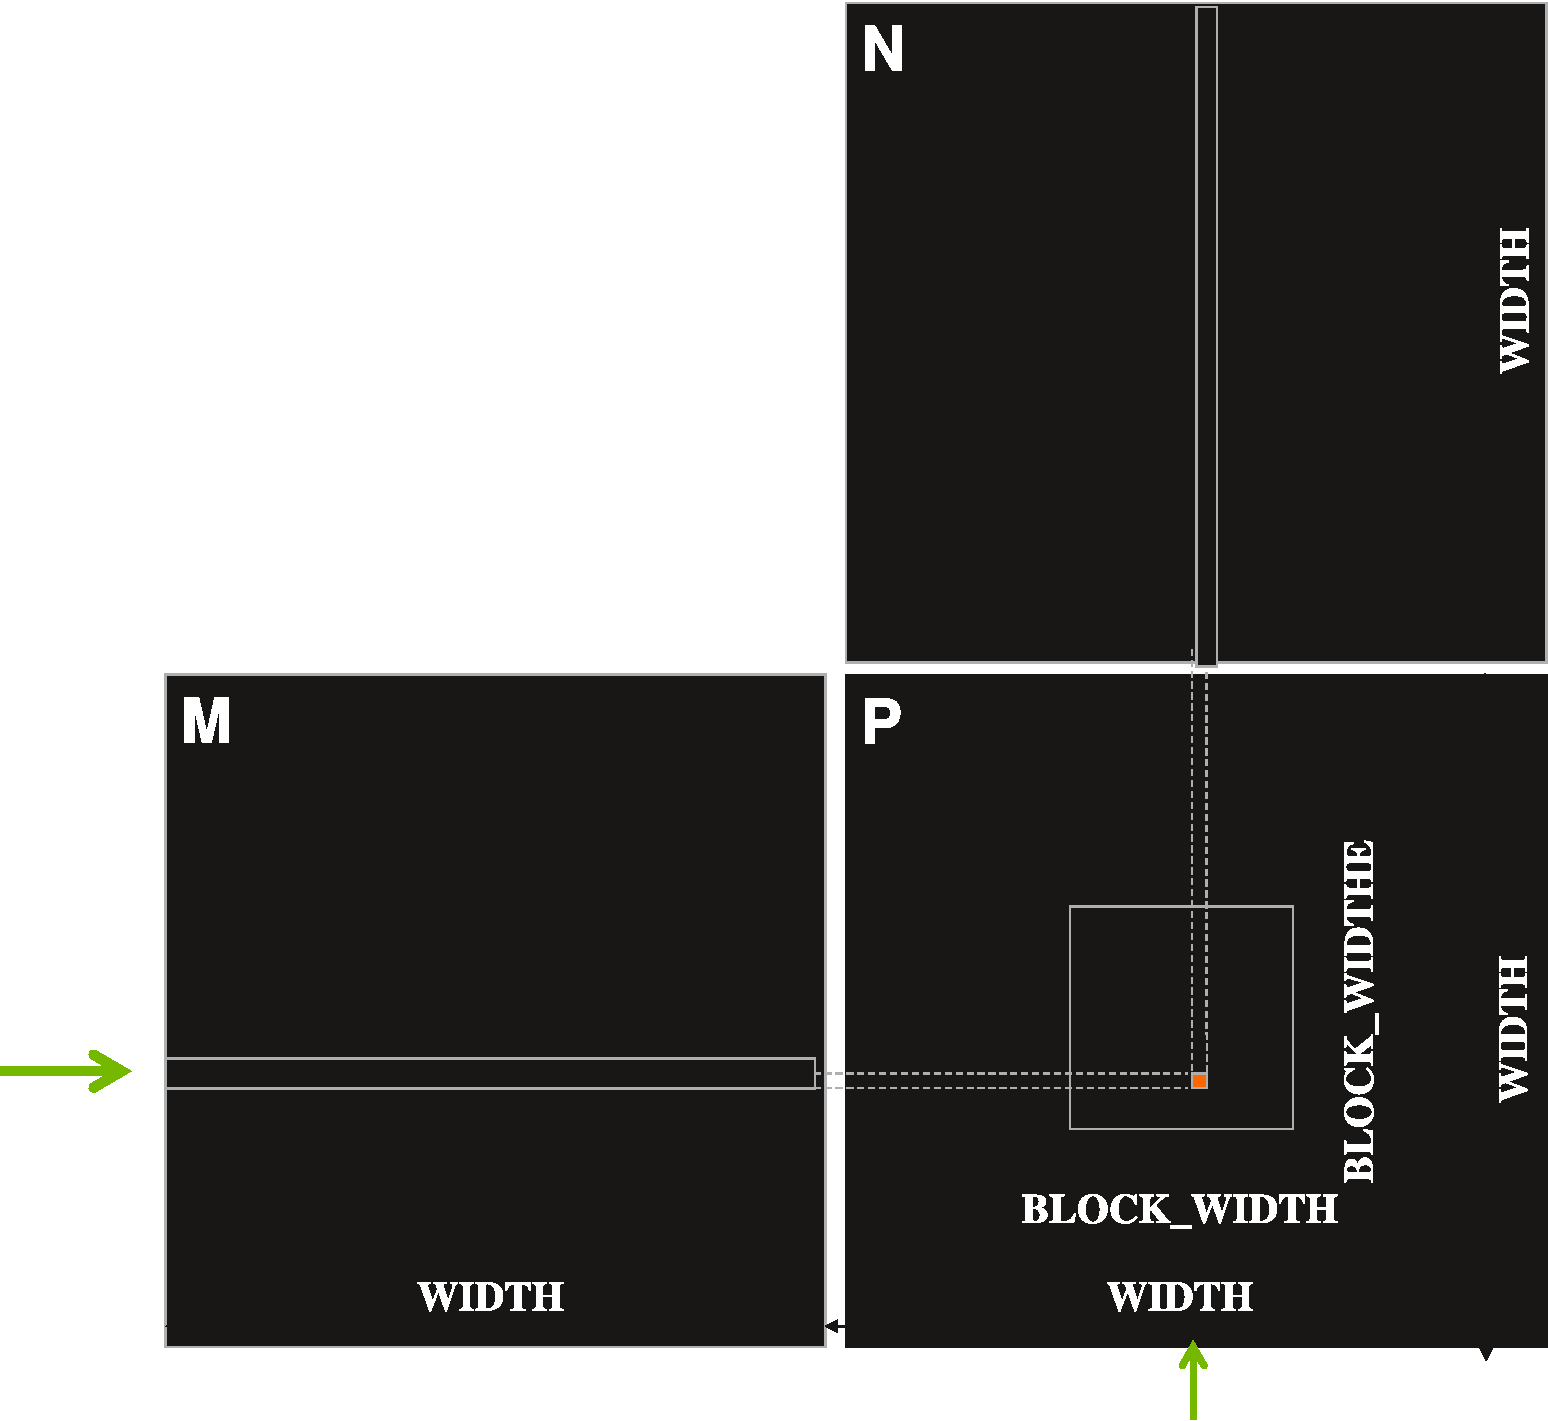
\includegraphics[width=.8\textwidth]{img/cuda-matrix-multiplication-1.pdf}
    \end{center}
    
    Arrows show the direction of data flow, indicating how elements from matrices $M$ and $N$ are multiplied to form matrix $P$.

    The code used to perform the matrix multiplication is as follows:
    \begin{lstlisting}[language=C++]
__global__ void MatrixMulKernel(
    float* M, float* N, float* P, int Width
) {
    // Calculate the row index of the P element and M
    int Row = blockIdx.y * blockDim.y + threadIdx.y; $\label{code: row index}$

    // Calculate the column index of P and N
    int Col = blockIdx.x * blockDim.x + threadIdx.x; $\label{code: col index}$

    int RowTimesWidth = Row * Width;

    if ((Row < Width) && (Col < Width)) {
        float Pvalue = 0;
        // Each thread computes one element
        // of the block sub-matrix
        for (int k = 0; k < Width; ++k) {
            Pvalue += M[RowTimesWidth + k] * 
                      N[k * Width + Col];
        }
        P[RowTimesWidth + Col] = Pvalue;
    }
}\end{lstlisting}
    \begin{itemize}
        \item The \texttt{MatrixMulKernel} function is defined to run on the GPU (indicated by \texttt{\_\_global\_\_}). It takes pointers to matrices $M$, $N$, $P$, and an integer \texttt{Width} representing the dimensions.

        \item Calculate Row Index (row \ref{code: row index}). It calculates the row index of the current element in matrix $P$ that the thread is responsible for.

        \item Calculate Column Index (row \ref{code: col index}). It calculates the column index of the current element in matrix $P$.
        
        \item The if condition ensures that the thread operates within the bounds of the matrices.
        
        \item If the condition is true, initializes the \texttt{Pvalue} and iterates over the row of $M$ and column of $N$. Each iteration accumulates the product of corresponding elements from $M$ and $N$.
        
        \item Finally, stores the computed value in matrix $P$.
    \end{itemize}
\end{examplebox}

\noindent
Since the previous example shows problems with \textbf{global memory access} (because accessing elements of matrices $M$, $N$, and $P$ involves global memory), \textbf{optimization} (it doesn't load elements into shared memory to reduce global memory accesses), and \textbf{data locality} (because consecutive threads don't access successive memory locations), we propose an alternative.

\begin{flushleft}
    \textcolor{Green3}{\faIcon{tools} \textbf{Alternative (better) implementation of the previous example}}
\end{flushleft}
The following figure shows how threads are mapped to elements of the output matrix $P$ during matrix multiplication. It shows how the matrix is divided into blocks and how threads handle these blocks.
\begin{figure}[!htp]
    \centering
    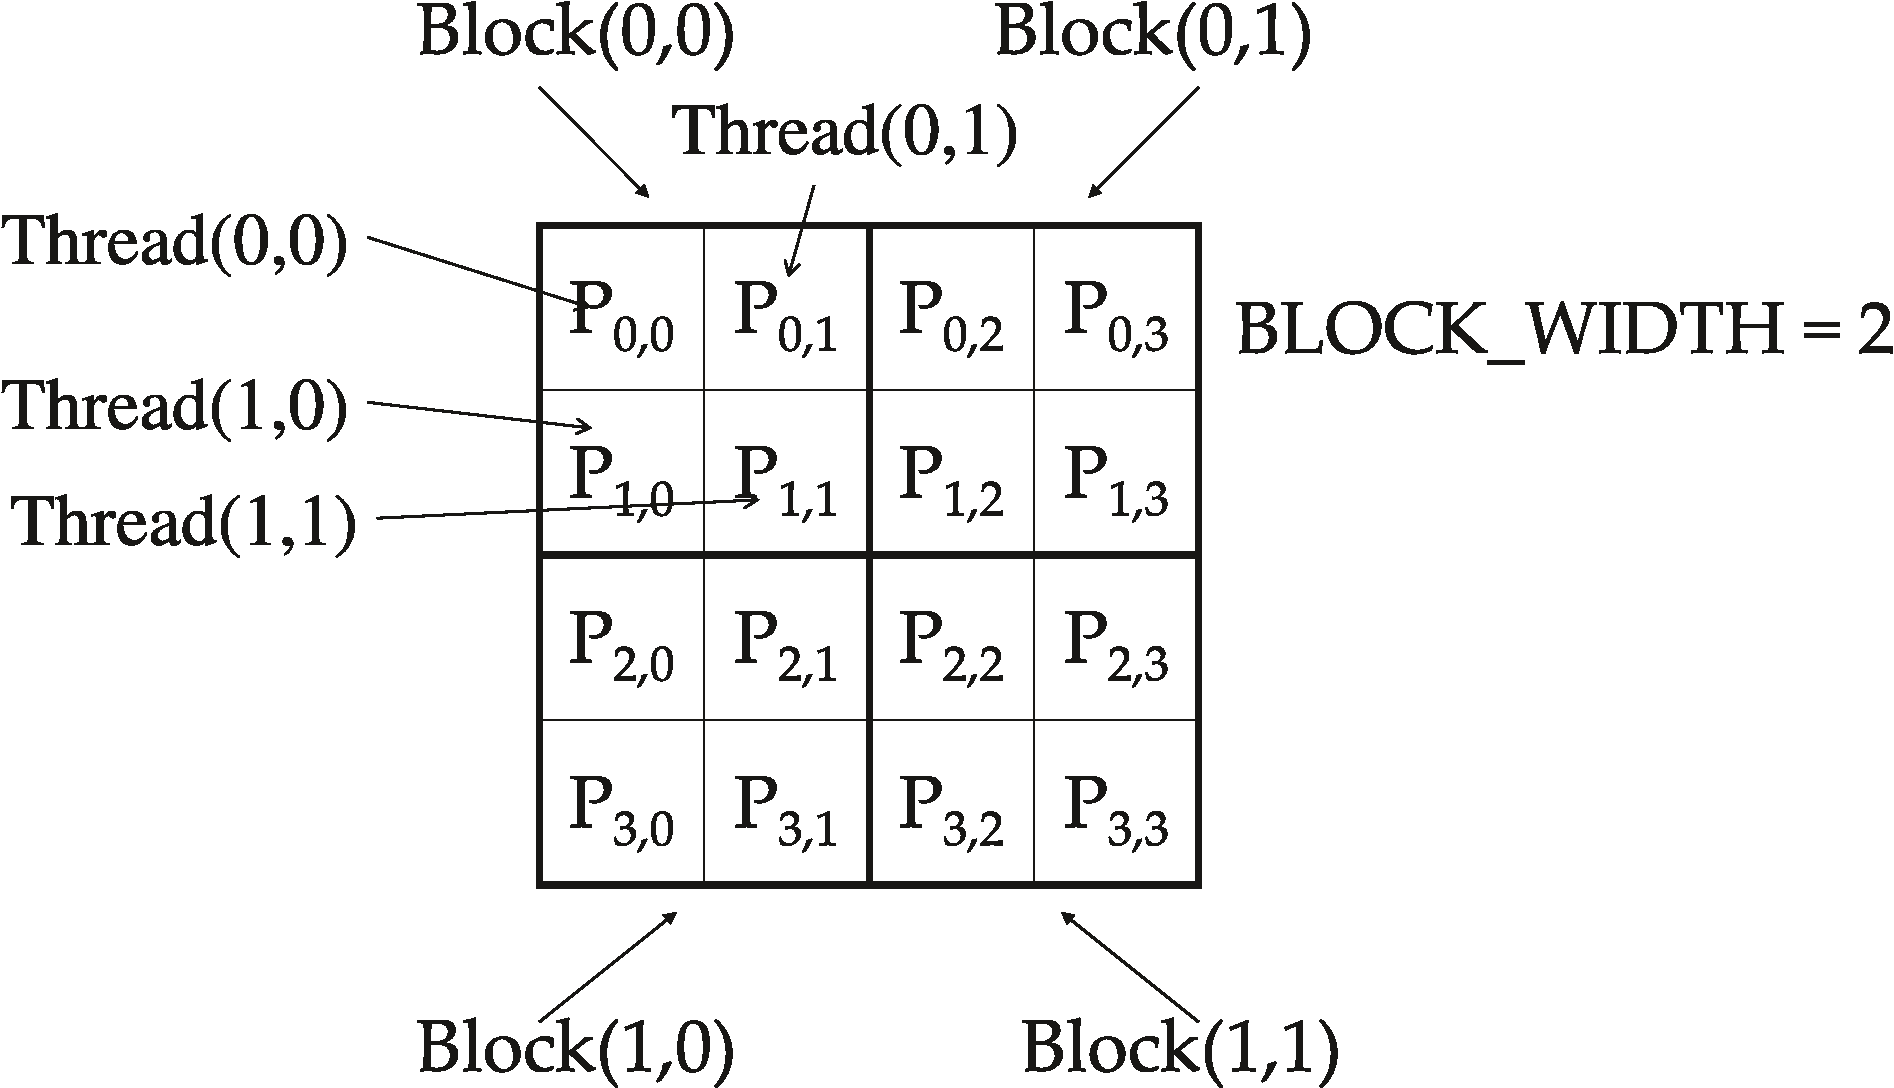
\includegraphics[width=.8\textwidth]{img/cuda-matrix-multiplication-2.pdf}
\end{figure}
\begin{itemize}
    \item The $4 \times 4$ matrix $P$ is divided into smaller $2 \times 2$ blocks. This division helps in managing data more efficiently and improves memory access patterns.
    \item The \texttt{BLOCK\_WIDTH} is 2, indicating that each block contains $2 \times 2$ elements.
    \item Each block of the matrix $P$ is assigned to a specific thread.
    \begin{itemize}
        \item Block(0,0) is handled by Thread(0,0).
        \item Block(0,1) is handled by Thread(0,1).
        \item Block(1,0) is handled by Thread(1,0).
        \item Block(1,1) is handled by Thread(1,1).
    \end{itemize}
\end{itemize}
The \textbf{mapping ensures that each thread is responsible for computing the values of a specific block} in matrix $P$.

\highspace
In the following figure, we illustrate an example of how elements $P_{0,0}$ and $P_{0,1}$ in matrix $P$ are calculated using elements from matrices $M$ and $N$.
\begin{figure}[!htp]
    \centering
    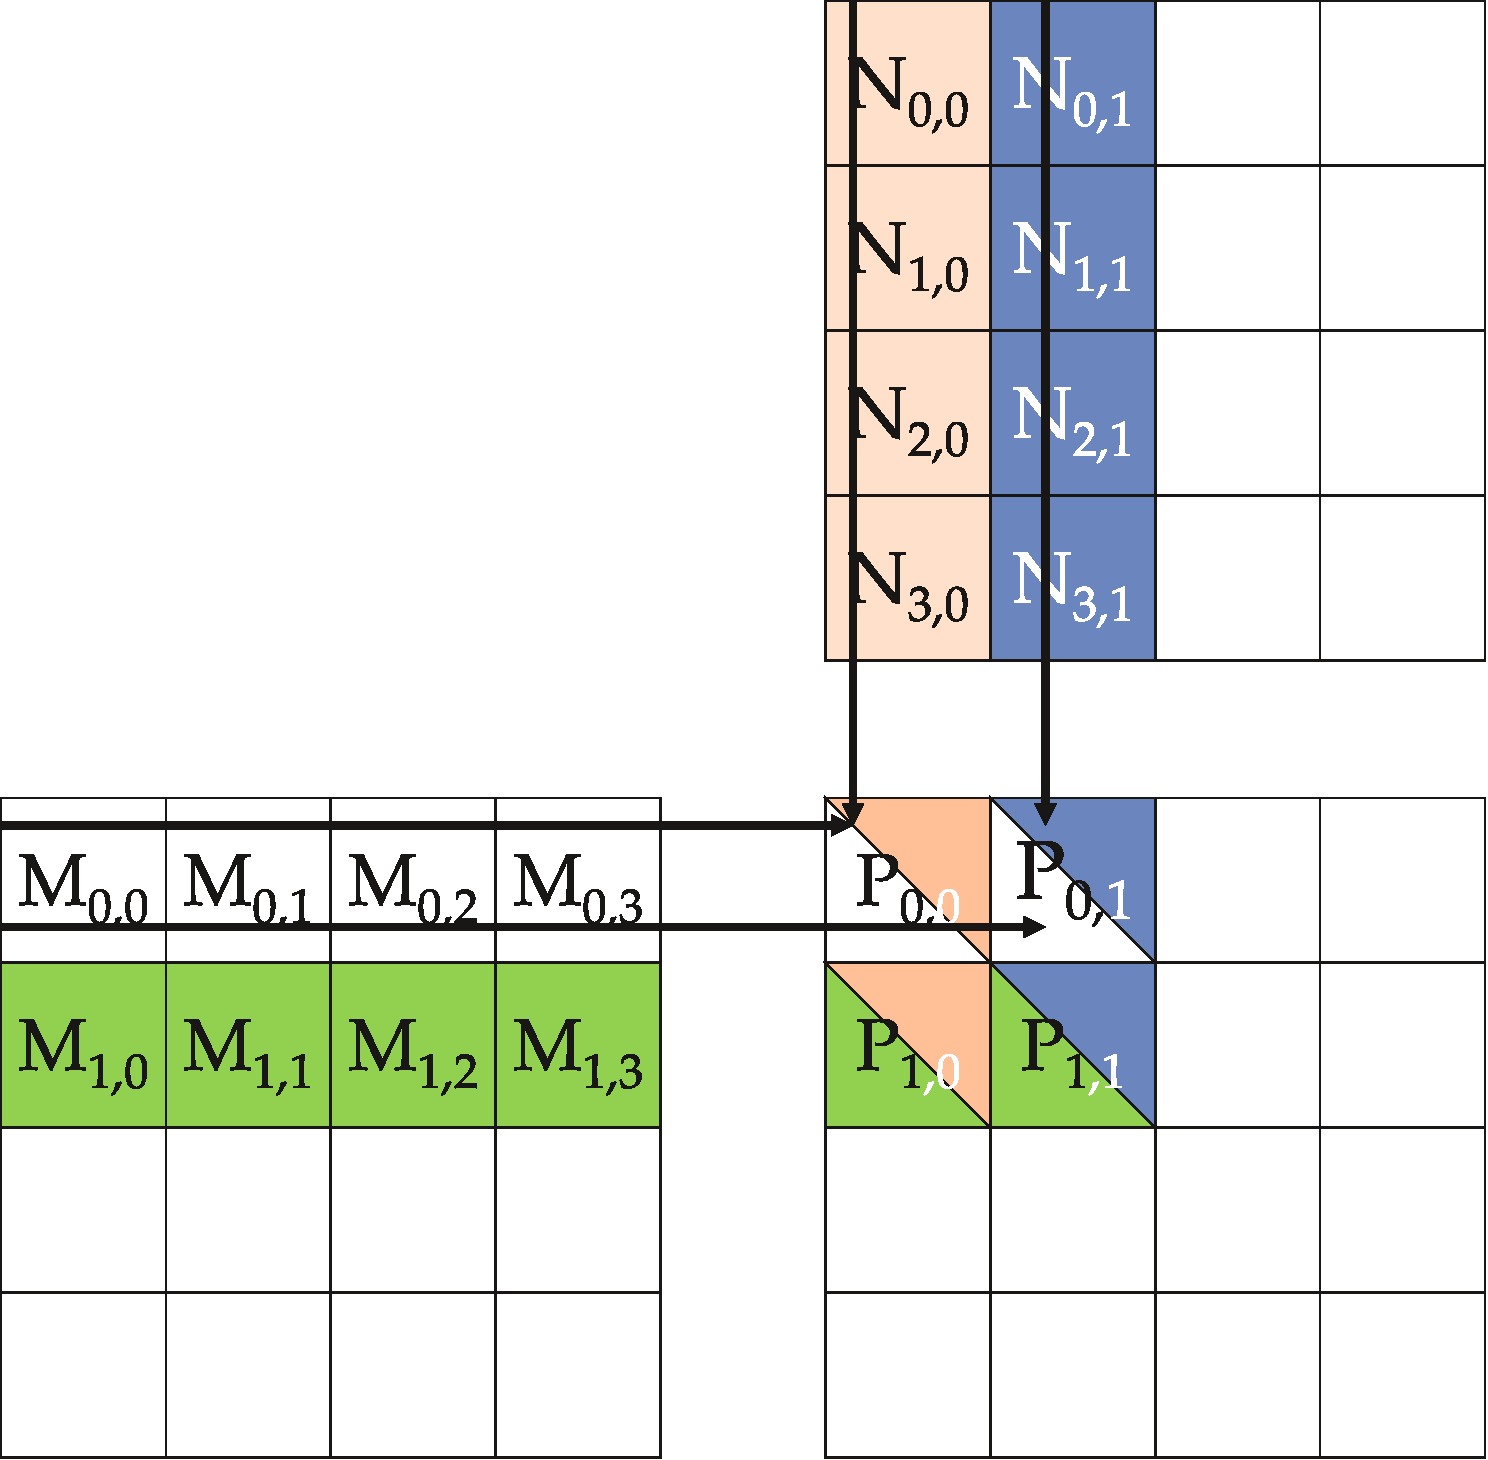
\includegraphics[width=.6\textwidth]{img/cuda-matrix-multiplication-3.pdf}
\end{figure}
\begin{itemize}
    \item To compute $P_{0,0}$, are used elements from:
    \begin{itemize}
        \item The first row of matrix $M$ $\left(M_{0,0}, M_{0,1}, M_{0,2}, M_{0,3}\right)$
        \item The first column of matrix $N$ $\left(N_{0,0}, N_{1,0}, N_{2,0}, N_{3,0}\right)$
    \end{itemize}
    
    The computation involves multiplying corresponding elements and summing the results:
    \begin{equation*}
        \begin{array}{rcl}
            P_{0,0} &=& (M_{0,0} \times N_{0,0}) + (M_{0,1} \times N_{1,0}) + \\ [.3em]
                     && (M_{0,2} \times N_{2,0}) + (M_{0,3} \times N_{3,0})
        \end{array}
    \end{equation*}


    \item To compute $P_{0,1}$, are used elements from:
    \begin{itemize}
        \item The first row of matrix $M$ $\left(M_{0,0}, M_{0,1}, M_{0,2}, M_{0,3}\right)$
        \item The second column of matrix $N$ $\left(N_{0,1}, N_{1,1}, N_{2,1}, N_{3,1}\right)$
    \end{itemize}
    
    The computation involves multiplying corresponding elements and summing the results:
    \begin{equation*}
        \begin{array}{rcl}
            P_{0,1} &=& (M_{0,0} \times N_{0,1}) + (M_{0,1} \times N_{1,1}) + \\ [.3em]
                     && (M_{0,2} \times N_{2,1}) + (M_{0,3} \times N_{3,1})
        \end{array}
    \end{equation*}
\end{itemize}
And \emph{\textbf{why is this related to storage and data locality?}} For three reasons:
\begin{enumerate}[label=\textcolor{Green3}{\faIcon{check}}]
    \item \textcolor{Green3}{\textbf{Memory Access Patterns}}. By dividing the matrix into \textbf{blocks and assigning specific threads to handle these blocks}, the computation can take advantage of memory locality. \textbf{Threads working on the same block will likely access contiguous memory locations}, which improves memory access efficiency.
 
    \item \textcolor{Green3}{\textbf{Shared Memory Usage}}. Instead of repeatedly accessing global memory, \textbf{threads can load the necessary block data into shared memory once}. All \textbf{threads in a block can then work on the data in shared memory}, significantly reducing global memory access and thus improving performance.
 
    \item \textcolor{Green3}{\textbf{Optimization for Performance}}. Reducing the number of global memory accesses by optimizing data locality and using shared memory can drastically improve the performance of the matrix multiplication kernel. Efficient \textbf{mapping of threads to data and making use of memory hierarchy are key strategies for achieving high performance in CUDA applications}.
\end{enumerate}

\begin{flushleft}
    \textcolor{Red2}{\faIcon{book} \textbf{Memory/Data Locality are fundamental, now we go deep}}
\end{flushleft}
Before explaining the keywords used by CUDA, it is important to understand the \textbf{programmer's view} of CUDA memory.

\begin{figure}[!htp]
    \centering
    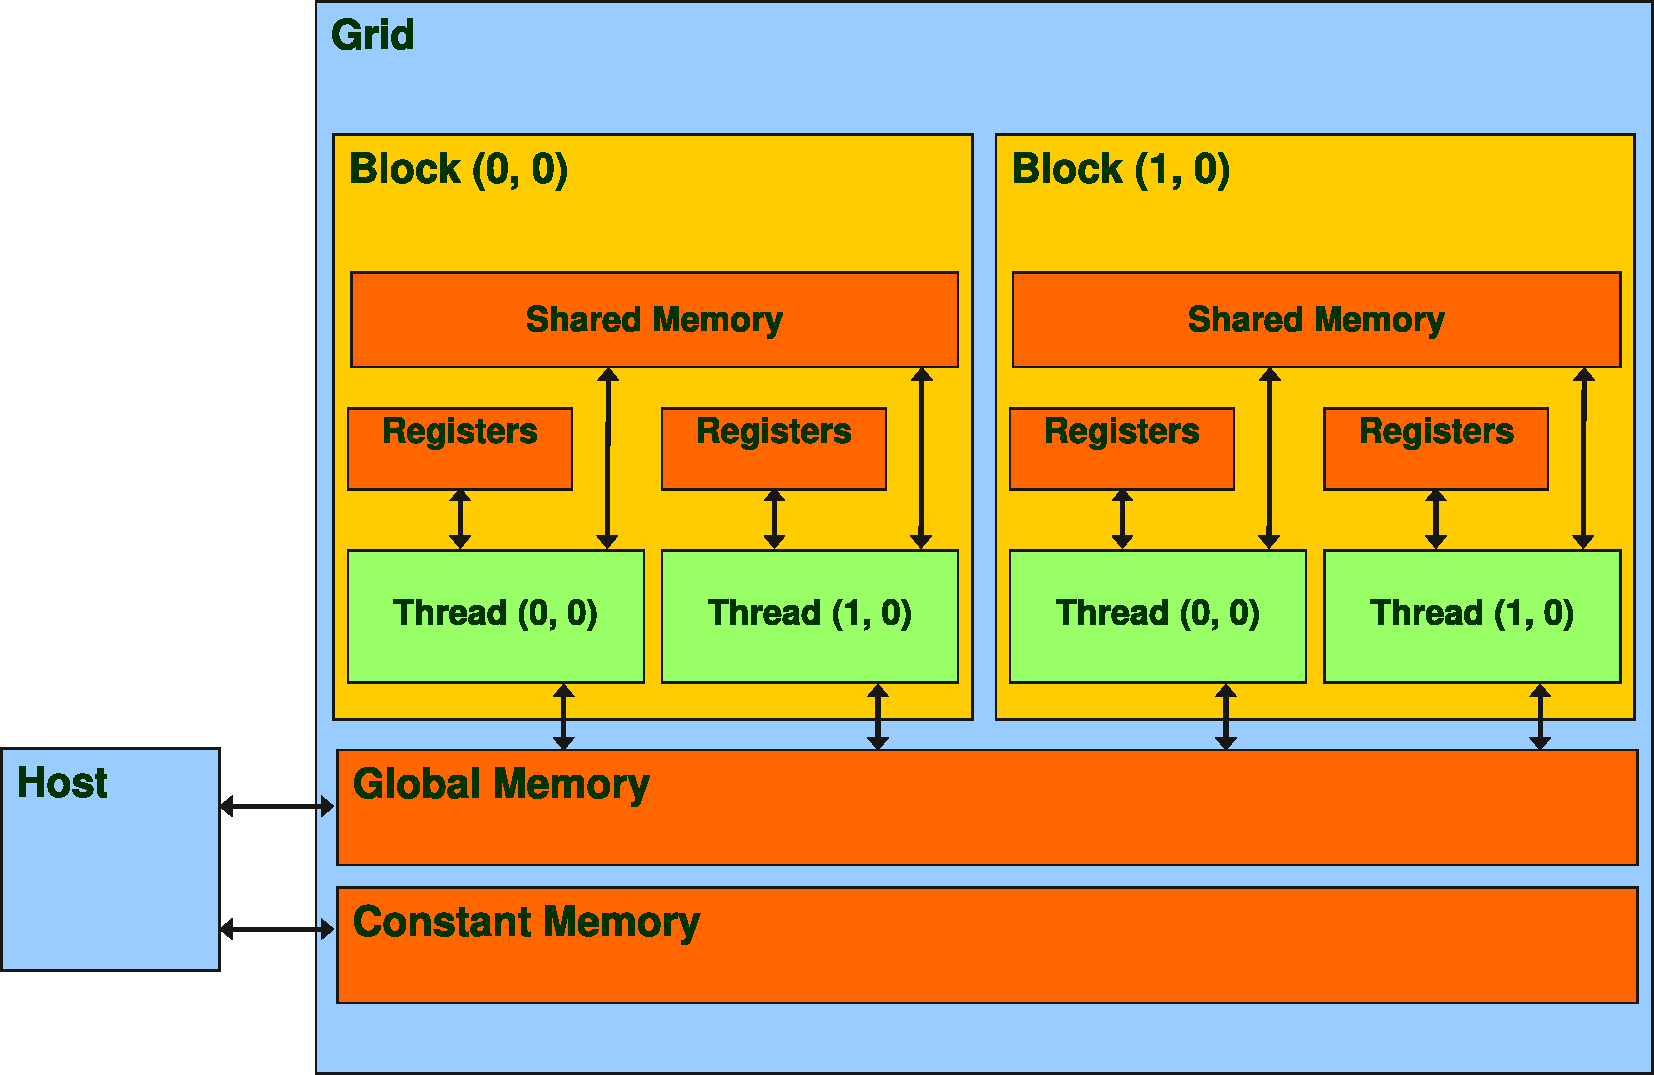
\includegraphics[width=\textwidth]{img/programmer-view-cuda-mem-1.pdf}
\end{figure}
\begin{itemize}
    \item \textbf{Host} (CPU) \textbf{Memory}. Connected to the GPU, but \emph{distinct} from GPU memory.
    \item \textbf{Global Memory}. Accessible by \emph{all threads} and the \emph{host}. It's the \emph{largest} but also the \emph{slowest} type of memory.
    \item \textbf{Constant Memory}. Read-only memory accessible by \emph{all} threads.
    \item \textbf{Grid}. Contains multiple blocks, each consisting of threads (we have already seen and discussed this in Section \ref{definition: CUDA Grids}, page \pageref{definition: CUDA Grids}).
    \item \textbf{Shared Memory}. Faster than global memory, shared among threads within the same block.
    \item \textbf{Registers}. The fastest memory, local to each thread.
\end{itemize}
CUDA has specific declarations for different types of memory:
\begin{itemize}
    \item \important{Local} \textbf{Variable} (\texttt{int LocalVar}): stored in registers, scope and lifetime are per thread.
    \item \important{Shared} \textbf{Variable} (\texttt{\_\_shared\_\_ int SharedVar}): stored in shared memory, scope and lifetime are per block.
    \item \important{Global} \textbf{Variable} (\texttt{\_\_device\_\_ int GlobalVar}): stored in global memory, scope is the entire grid, and the lifetime is the duration of the application.
    \item \important{Constant} \textbf{Variable} (\texttt{\_\_constant\_\_ int ConstantVar}): stored in constant memory, scope is the grid, and the lifetime is the duration of the application.
\end{itemize}
\begin{table}[!htp]
    \centering
    \begin{tabular}{@{} l c c c @{}}
        \toprule
        \textbf{Variable Declaration} & \textbf{Memory} & \textbf{Scope} & \textbf{Lifetime} \\
        \midrule
        \texttt{int LocalVar} & Register & Thread & Thread \\
        \texttt{\_\_shared\_\_ int SharedVar} & Shared & Block & Block \\
        \texttt{\_\_device\_\_ int GlobalVar} & Global & Grid & Application \\
        \texttt{\_\_constant\_\_ int ConstantVar} & Constant & Grid & Application \\
        \bottomrule
    \end{tabular}
    \caption{CUDA Memory Types, Scope, and Lifetime.}
    \label{table: CUDA Memory Types, Scope, and Lifetime}
\end{table}

\noindent
There are two observations to make:
\begin{enumerate}
    \item The \texttt{\_\_device\_\_} keyword is \textbf{optional} when used with \texttt{\_\_shared\_\_} or \texttt{\_\_constant\_\_}.


    \item The \textbf{automatic variables} (those that are automatically managed by the compiler) \textbf{reside in the registers} because they are the fastest type of memory available to threads (very close to the processor).
    
    However, there's an \textbf{exception for per-thread arrays}: when we declare an array inside a kernel function, this array is unique to each thread and can be relatively large. Due to their size and potential complexity, these \textbf{per-thread arrays cannot fit in registers and are stored in global memory instead}.
\end{enumerate}

\begin{flushleft}
    \textcolor{Green3}{\faIcon{question-circle} \textbf{And how do I decide where to put the variables?}}
\end{flushleft}
It depends on the implementation. The good question to ask is: \emph{can the host access the declared variable?}
\begin{itemize}
    \item If the \textbf{host can access the variable}, it should be a \texttt{global} or \texttt{constant} variable.
    \begin{itemize}
        \item Declared outside of a function;
        \item Accessible by both host (CPU) and device (GPU).
    \end{itemize}

    \item If the \textbf{host cannot access the variable}, it should be a \texttt{register} or \texttt{shared} variable.
    \begin{itemize}
        \item Declared inside the kernel function;
        \item If it is \texttt{shared}, it is accessible to all threads within the same block;
        \item On the other hand, if it is \texttt{register} (local), it is only accessible to individual threads, suitable for frequently accessed variables.
    \end{itemize}
\end{itemize}

\highspace
\begin{flushleft}
    \textcolor{Red2}{\faIcon{bookmark} \textbf{In-depth analysis of shared memory in CUDA}}
\end{flushleft}
Some features of shared memory in CUDA:
\begin{enumerate}
    \item \important{Shared Memory in Each Streaming Multiprocessor (SM)}. Each SM in a CUDA GPU has its own shared memory.
    
    Shared memory is significantly faster than global memory, both in terms of latency and throughput.
    
    
    \item \important{Scope and Lifetime}. The scope of shared memory is limited to the block; only threads within the same block can access the same shared memory.
    
    The lifetime of shared memory is tied to the thread block's lifetime. Once the block finishes execution, the shared memory is released.
    
    
    \item \important{Access}. Shared memory is accessed using memory load/store instructions.
    
    It acts as a scratchpad memory in the computer architecture, allowing threads to quickly share and exchange data.
\end{enumerate}
\begin{figure}[!htp]
    \centering
    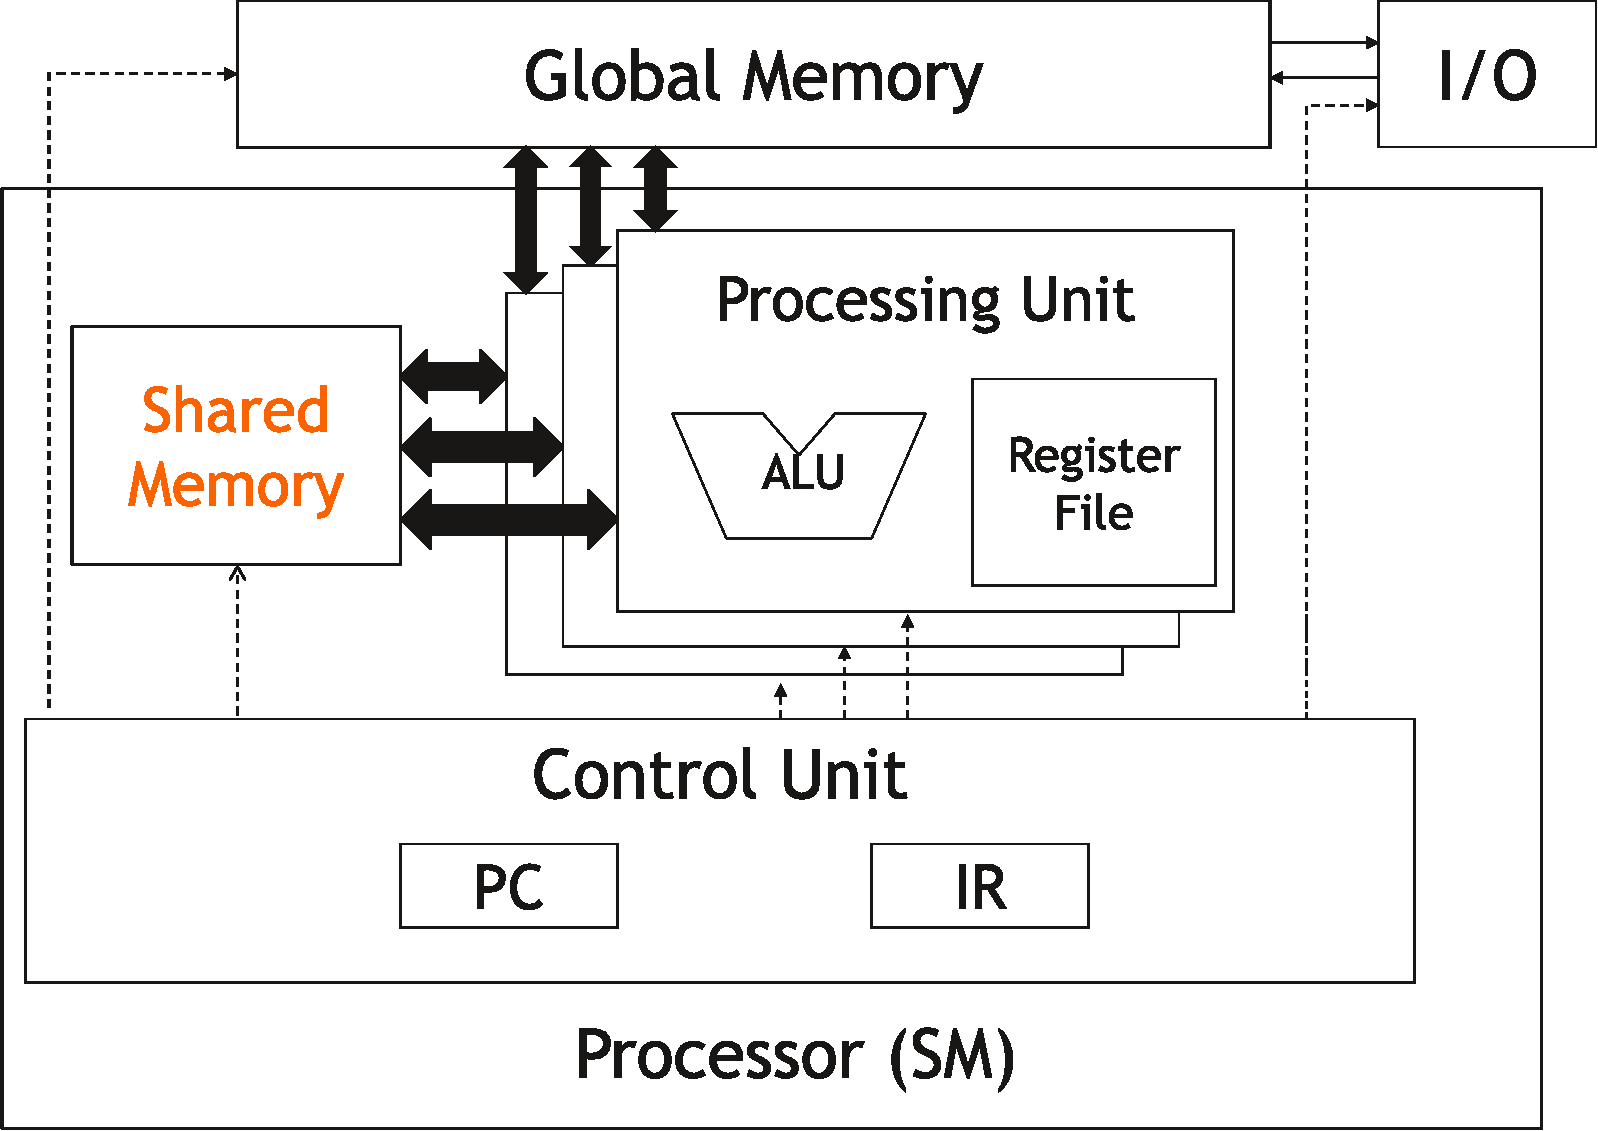
\includegraphics[width=.8\textwidth]{img/cuda-shared-memory-1.pdf}
    \caption{Hardware View of CUDA Memories.}
\end{figure}
\begin{itemize}
    \item \textbf{Global Memory}. A large memory space accessible by all threads and the host (CPU). Used for data storage and retrieval but has higher latency compared to shared memory.

    \item \textbf{Shared Memory}. A smaller, faster memory space within each SM. Used for data sharing among threads in the same block.

    \item \textbf{Processing Unit}.Contains Arithmetic Logic Units (ALUs) and a Register File for performing computations. Registers are the fastest type of memory, used for storing per-thread data.

    \item \textbf{Control Unit}. Manages the execution of instructions, including the Program Counter (PC) and Instruction Register (IR).

    \item \textbf{I/O}. Represents input/output operations.
\end{itemize}